%!TEX root = ../dissertation.tex
\section{Representation of eye orientation in 3 dimensions}
\label{cha2:represent}
In computer vision, it's customary to use the coordinate system on the left of Figure \ref{cha2:sec2:fig:coordsys2}, but in neuroscience a different convention, represented on the right of the Figure, is used. In order to be coherent with computer vision concepts, the first mentioned convention will be the one in use throughout the remaining of this section.

\begin{figure}[!htb]
	\centering
	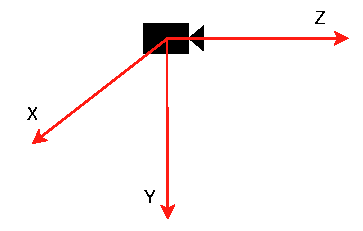
\includegraphics[width=0.41\textwidth]{images/cvcoordinatesys.pdf}
	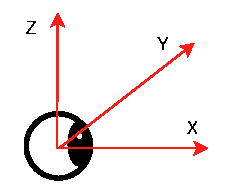
\includegraphics[width=0.25\textwidth]{images/cvcoordinatesysq.pdf}
	\caption[Computer Vision vs Neuroscience coordinate systems]{On the left, the coordinate system used in computer vision with the torsional component coming out of the front of the camera. On the right, the coordinate system used in the neuroscience field with the torsional component coming out of the front of the eye.}
	\label{cha2:sec2:fig:coordsys2}
\end{figure}

There are several ways of representing a rotation in 3D, the most common being Euler angles and rotation matrices. Euler angles are three angles that describe the orientation of a rigid body with respect to a fixed coordinate system. For this work, maintaining the coordinate system said above, the sequence of rotations used to represent a given orientation can be defined by the angles $[\theta_Z \ \theta_Y \ \theta_X]$, which corresponds to rotating around Z, Y, X axes, respectively.

\subsection{Rotation matrices}
\label{rotmatsss}
The human eye is a purely rotative body (no translations), and thus any orientation can be described by a unique series of three rotations around each of the axis defined in three dimensional space as
\begin{equation}
\label{rrr}
R _ { z } ( \theta_Z ) = \left[ \begin{array} { c c c } { \cos \theta_Z } & { - \sin \theta_Z } & { 0 } \\ { \sin \theta_Z } & { \cos \theta_Z } & { 0 } \\ { 0 } & { 0 } & { 1 } \end{array} \right], \
R _ { y } ( \theta_Y ) = \left[ \begin{array} { c c c } { \cos \theta_Y } & { 0 } & { \sin \theta_Y } \\ { 0 } & { 1 } & { 0 } \\ { - \sin \theta_Y } & { 0 } & { \cos \theta_Y } \end{array} \right], \
R _ { x } ( \theta_X ) = \left[ \begin{array} { c c c } { 1 } & { 0 } & { 0 } \\ { 0 } & { \cos \theta_X } & { - \sin \theta_X } \\ { 0 } & { \sin \theta_X } & { \cos \theta_X} \end{array} \right],
\end{equation}
where each angle is defined in counter-clockwise direction around each axis. An arbitrary rotation, $R$, may then be defined as some multiplication (i.e. a serial order) of those three, noting that the order by which they are multiplied matters (rotations are non-commutative). A matrix originated from any combination of those is a rotation matrix because it satisfies the following conditions,
\begin{align}
	R^{-1} = R^T\\
	det(R) = 1.
\end{align} 

Instead of using multiple rotations done after each other around three different axes, Euler's theorem states that the orientation of the rotating body can also be parametrized by a single rotation with an angle, $\rho$, about an axis in 3D, $\hat{\mathbf{n}} = (n_1, n_2, n_3)$. That rotation is denoted as $R(\hat{\mathbf{n}}, \rho)$ and is given by 
\begin{equation}
R ( \hat { \mathbf{n} } , \rho ) = \left( \begin{array} { c c c } { \cos \rho + n _ { 1 } ^ { 2 } ( 1 - \cos \rho ) } & { n _ { 1 } n _ { 2 } ( 1 - \cos \rho ) - n _ { 3 } \sin \rho } & { n _ { 1 } n _ { 3 } ( 1 - \cos \rho ) + n _ { 2 } \sin \rho } \\ { n _ { 1 } n _ { 2 } ( 1 - \cos \rho ) + n _ { 3 } \sin \rho } & { \cos \rho + n _ { 2 } ^ { 2 } ( 1 - \cos \rho ) } & { n _ { 2 } n _ { 3 } ( 1 - \cos \rho ) + n _ { 2 } \sin \rho } \\ { n _ { 1 } n _ { 3 } ( 1 - \cos \rho ) - n _ { 2 } \sin \rho } & { n _ { 2 } n _ { 3 } ( 1 - \cos \rho ) + n _ { 1 } \sin \rho } & { \cos \rho + n _ { 3 } ^ { 2 } ( 1 - \cos \rho ) } \end{array} \right).
\end{equation}

Still, rotation matrices are not the most efficient way to define rotations given they have nine elements and only three are actually necessary to describe the rotation uniquely. Hence, in oculomotor literature more suitable representations are used, such as quaternions, or rotation vectors that are more intuitive. \cite{rep}\cite{mathrot}

\subsection{Quaternions}
\label{cha2:represent:quat}
Quaternions are 4-dimensional complex algebraic objects that are related to a rotation around an axis, $\hat{ \mathbf{n}}$ by an angle $\rho$ as follows,
\begin{equation}
\label{sec2:eq:q}
q = \cos ( \rho / 2 ) + \mathbf{i} \sin ( \rho / 2 ) \mathbf{\hat{n}} \equiv q _ { 0 } + {\bf i}\cdot  {\bf q},
\end{equation}
where $q_0$ and $\mathbf{q} = [q_1 \ q_2 \ q_3]$ are the scalar and vectorial parts of the quaternion, respectively, and ${\bf i}$ is the complex 3D vector. 

Like rotation matrices, a quaternion can be defined as a sequence of rotations by multiplying each corresponding quaternion in sequence.
The product of a quaternion $\mathbf{q}$ with a quaternion $\mathbf{p}$ is 
\begin{equation}
	q_0 p_0 - \mathbf{q} \cdot \mathbf{p} + q_0 \mathbf{p} + p_0 \mathbf{q} + \mathbf{q} \times \mathbf{p}.
\end{equation}
The rotation between two quaternions can be obtained by 
\begin{equation}
\mathbf{p} \cdot \mathbf{q}^{-1},
\end{equation}
where $\mathbf{q}^{-1} = \frac{q^*}{|q|}$ with $q^*$ being the conjugate of $q$.

Moreover, quaternions can be related to rotation matrices through
\begin{equation}
	R=\left[\begin{array}{lll}{1-2\left(q_{2}^{2}+q_{3}^{2}\right)} & {2\left(q_{1} q_{2}-q_{0} q_{3}\right)} & {2\left(q_{1} q_{3}+q_{0} q_{2}\right)} \\ {2\left(q_{1} q_{2}+q_{0} q_{3}\right)} & {1-2\left(q_{1}^{2}+q_{3}^{2}\right)} & {2\left(q_{2} q_{3}-q_{0} q_{1}\right)} \\ {2\left(q_{1} q_{3}-q_{0} q_{2}\right)} & {2\left(q_{2} q_{3}+q_{0} q_{1}\right)} & {1-2\left(q_{1}^{2}+q_{2}^{2}\right)}\end{array}\right]
\end{equation}

For the description of eye movements, only the vectorial part, $\mathbf{q}$, is necessary, since the scalar part does not contain any information not already given by the vectorial one. Thus, it can be eliminated by using rotation vectors, which are related to quaternions  by $ \mathbf{r}  = {\bf q} / q _ { 0 }$.

\subsection{Rotation vector in head-fixed coordinates}
\label{killme}

The rotation vector, $\mathbf{r}$, is directed along the rotation axis, $\hat{\mathbf{n}}$, and its length varies with the amount of rotation, $\rho$, around it. It can be described by 
\begin{equation}
\mathbf{r} = \tan (\frac{\rho}{2}) \hat{ \mathbf{n}},
\end{equation}
where $\hat{ \mathbf{n}}$ can be obtained through a rotation matrix as
\begin{equation}
\label{sec2:eq:n}
\begin{aligned} 
n_ { 1 } & = \sin \rho \left( R _ { 32 } - R _ { 23 } \right) / 2  \\ 
n _ { 2 } & = \sin \rho \left( R _ { 13 } - R _ { 31 } \right) / 2  \\ 
n _ { 3 } & = \sin \rho \left( R _ { 21 } - R _ { 12 } \right) / 2 ,
\end{aligned}
\end{equation}
and $\rho$ through
\begin{equation}
\cos \rho = 1 / 2 \cdot \left( R _ { 11 } + R _ { 22 } + R _ { 33 } - 1 \right).
\end{equation}
It's important to note that in this format, the units are given in half-radians.
